
\subsection{Objectives of the analysis}
The analysis checks that students are matched with internships based on their skills and the requirements of the internship, making sure each student is only assigned to one internship. It also ensures that both students and companies are available at the same time for interviews and that no student is assigned to more than one internship. The internships follow a set process from creation to completion, and students' complaints and company details are kept confidential.



\subsection{Alloy Code}

module StudentsAndCompanies\\

\begin{verbatim}
-- Entities
\end{verbatim}\\
sig Student \{ \\
  skills: set Skill,         // Skills that the student has \\
  availability: set TimeSlot, \begin{verbatim}
-- Time slots when the student is available
\end{verbatim}\\
  complaints: set Complaint   \begin{verbatim}
-- Complaints filed by the student
\end{verbatim}\\
\} \\

sig Company \{ \\
  requirements: set Skill,   \begin{verbatim}
-- Skills required by the company for internships
\end{verbatim}\\
  internships: set Internship, \begin{verbatim}
-- Internships offered by the company
\end{verbatim}\\
  availability: set TimeSlot  \begin{verbatim}
-- Time slots when the company is available
\end{verbatim}\\
\} \\

sig Internship \{ \\
  requiredSkills: set Skill, \begin{verbatim}
-- Skills required for the internship
\end{verbatim}\\
  assigned: lone Student      \begin{verbatim}
-- Student assigned to the internship
\end{verbatim}\\
\} \\

sig University \{ \\
  complaintsReceived: set Complaint \begin{verbatim}
-- Complaints received by the university
\end{verbatim}\\
\} \\

sig Skill \{\} \\
sig TimeSlot \{\} \\
sig Complaint \{ \\
  student: one Student,       \begin{verbatim}
-- Student who filed the complaint
\end{verbatim}\\
  company: one Company        \begin{verbatim}
-- Company related to the complaint
\end{verbatim}\\
\} \\

\begin{verbatim}
-- Predicates for checking conditions
\end{verbatim}\\
pred validMatch[s: Student, i: Internship] \{ \\
  some s.skills \& i.requiredSkills \begin{verbatim}
-- Ensure student’s skills match internship requirements
\end{verbatim}\\
\} \\

pred uniqueMatch[s: Student, i: Internship] \{ \\
  i.assigned = s and no other: Internship | other.assigned = s \begin{verbatim}
-- Ensure no student is assigned to multiple internships
\end{verbatim}\\
\} \\

pred validAvailability[s: Student, c: Company] \{ \\
  some s.availability \& c.availability \begin{verbatim}
-- Ensure there’s an overlap in available time slots
\end{verbatim}\\
\} \\

pred validComplaintHandling[c: Complaint] \{ \\
  c in University.complaintsReceived \begin{verbatim}
-- Ensure complaints are received and handled by the university
\end{verbatim}\\
\} \\

\begin{verbatim}
-- Integrity constraints
\end{verbatim}\\
fact Integrity \{ \\
  \begin{verbatim}
-- Students cannot be assigned to multiple internships simultaneously
\end{verbatim}\\
  all s: Student | lone i: Internship | i.assigned = s => uniqueMatch[s, i] \\

  \begin{verbatim}
-- Internships should have required skills
\end{verbatim}\\
  all i: Internship | some i.requiredSkills \\

  \begin{verbatim}
-- All complaints should be handled by the university
\end{verbatim}\\
  all c: Complaint | validComplaintHandling[c] \\

  \begin{verbatim}
-- Availability for interviews should be agreed upon by both student and company
\end{verbatim}\\
  all s: Student, c: Company | validAvailability[s, c] \\
\} \\

\begin{verbatim}
-- Internship lifecycle stages
\end{verbatim}\\
abstract sig InternshipStage \{\} \\
one sig Created, Matched, Interviewed, Completed extends InternshipStage \{\} \\

sig InternshipLifecycle \{ \\
  internship: one Internship, \begin{verbatim}
-- Internship related to the lifecycle stage
\end{verbatim}\\
  stage: one InternshipStage  \begin{verbatim}
-- Current stage of the internship
\end{verbatim}\\
\} \\

fact LifecycleOrder \{ \\
  \begin{verbatim}
-- Ensure that the internship lifecycle follows the correct order: Created -> Matched -> Interviewed -> Completed
\end{verbatim}\\
  all lc: InternshipLifecycle | \\
    lc.stage = Completed => lc.stage in Interviewed + Matched + Created \\
\} \\

\begin{verbatim}
-- Data confidentiality checks
\end{verbatim}\\
fact Confidentiality \{ \\
  \begin{verbatim}
-- Ensure students' complaints are not accessible by other students
\end{verbatim}\\
  all s1, s2: Student | s1 != s2 => no s1.complaints \& s2.complaints \\

  \begin{verbatim}
-- Ensure companies cannot access each other's internships
\end{verbatim}\\
  all c1, c2: Company | c1 != c2 => no c1.internships \& c2.internships \\
\} \\

\begin{verbatim}
-- Interviewing stage ensures that both the company and the student are available
\end{verbatim}\\
sig Interview\\ \{
  student: one Student, \\
  company: one Company, \\
  timeSlot: one TimeSlot \\
\}


\begin{verbatim}
-- Predicates to validate each process
\end{verbatim}\\
pred ValidMatching \{ \\
  all s: Student, i: Internship | validMatch[s, i] \begin{verbatim}
-- Check that all student-internship matches are valid
\end{verbatim}\\
\} \\

pred UniqueAssignment \{ \\
  all s: Student | lone i: Internship | (i.assigned = s) implies uniqueMatch[s, i] \begin{verbatim}
-- Ensure no student is assigned to more than one internship
\end{verbatim}\\
\} \\

pred ScheduleConflict \{ \\
  all s: Student, c: Company | validAvailability[s, c] \begin{verbatim}
-- Ensure no scheduling conflicts between student and company
\end{verbatim}\\
\} \\

pred ComplaintHandling \{ \\
  all c: Complaint | validComplaintHandling[c] \begin{verbatim}
-- Ensure all complaints are handled
\end{verbatim}\\
\} \\

\begin{verbatim}
-- Running checks to validate the system
\end{verbatim}\\
run ValidMatching for 5 \\
run UniqueAssignment for 5 \\
run ScheduleConflict for 5 \\
run ComplaintHandling for 5


\begin{sidewaysfigure}
\centering
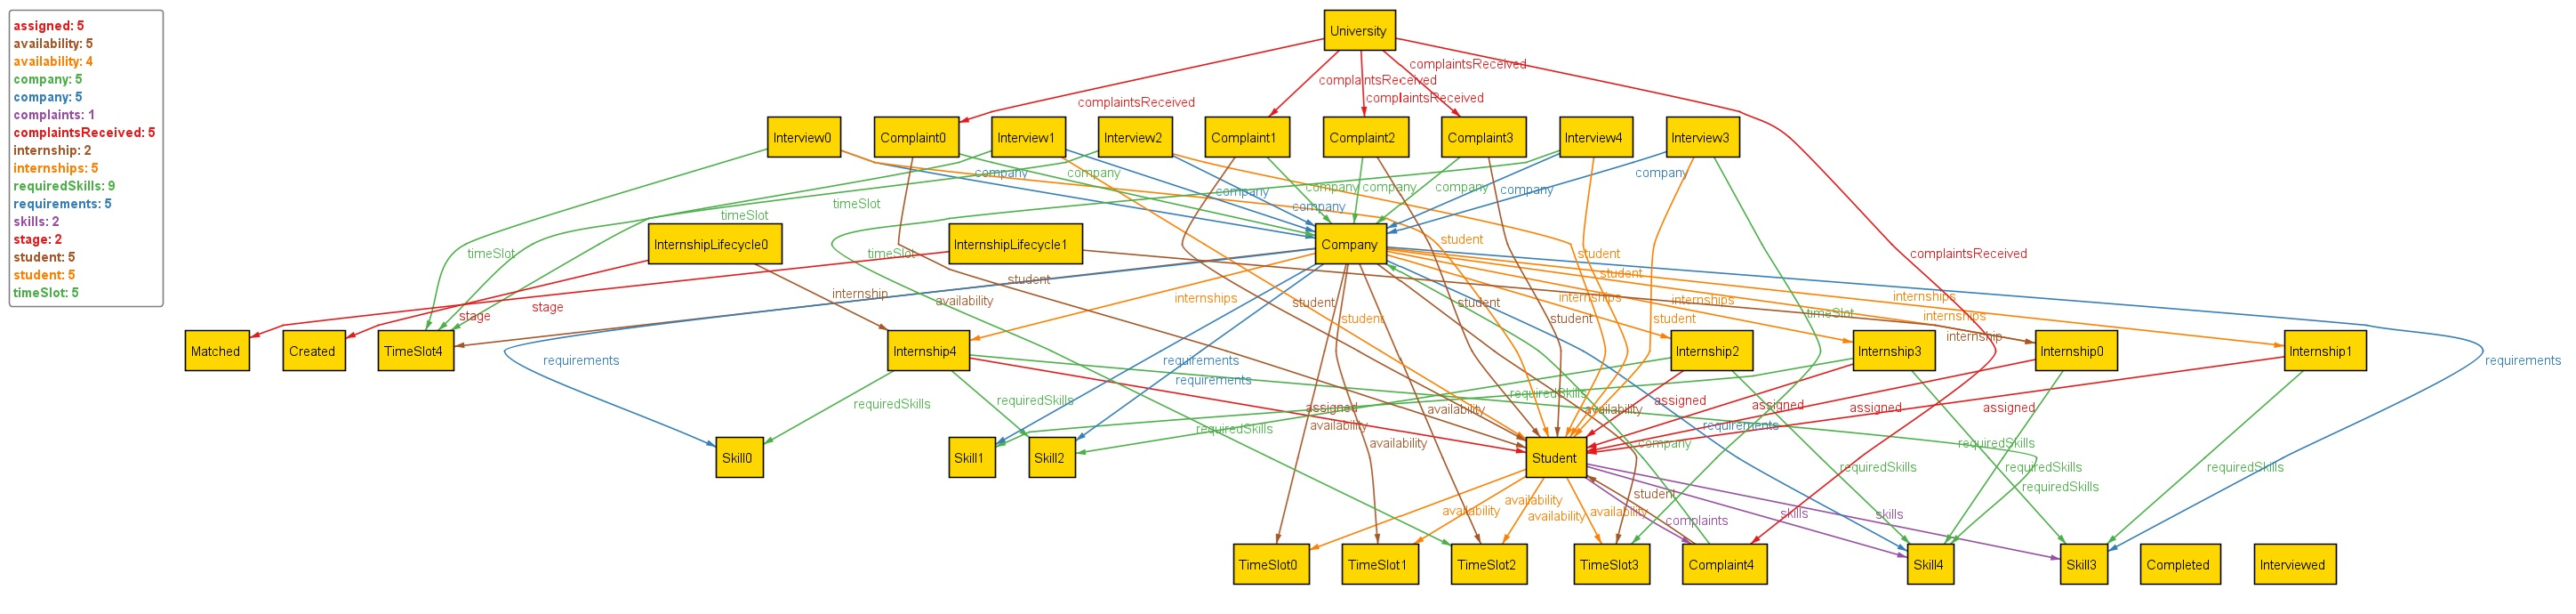
\includegraphics[width=\textwidth, angle=0]{Images/Alloy.jpg}
\caption{\label{fig:metamodel}Alloy solver visualization for the ValidMatching predicate.}
\end{sidewaysfigure}

\begin{figure}
\centering
\rotatebox{90}{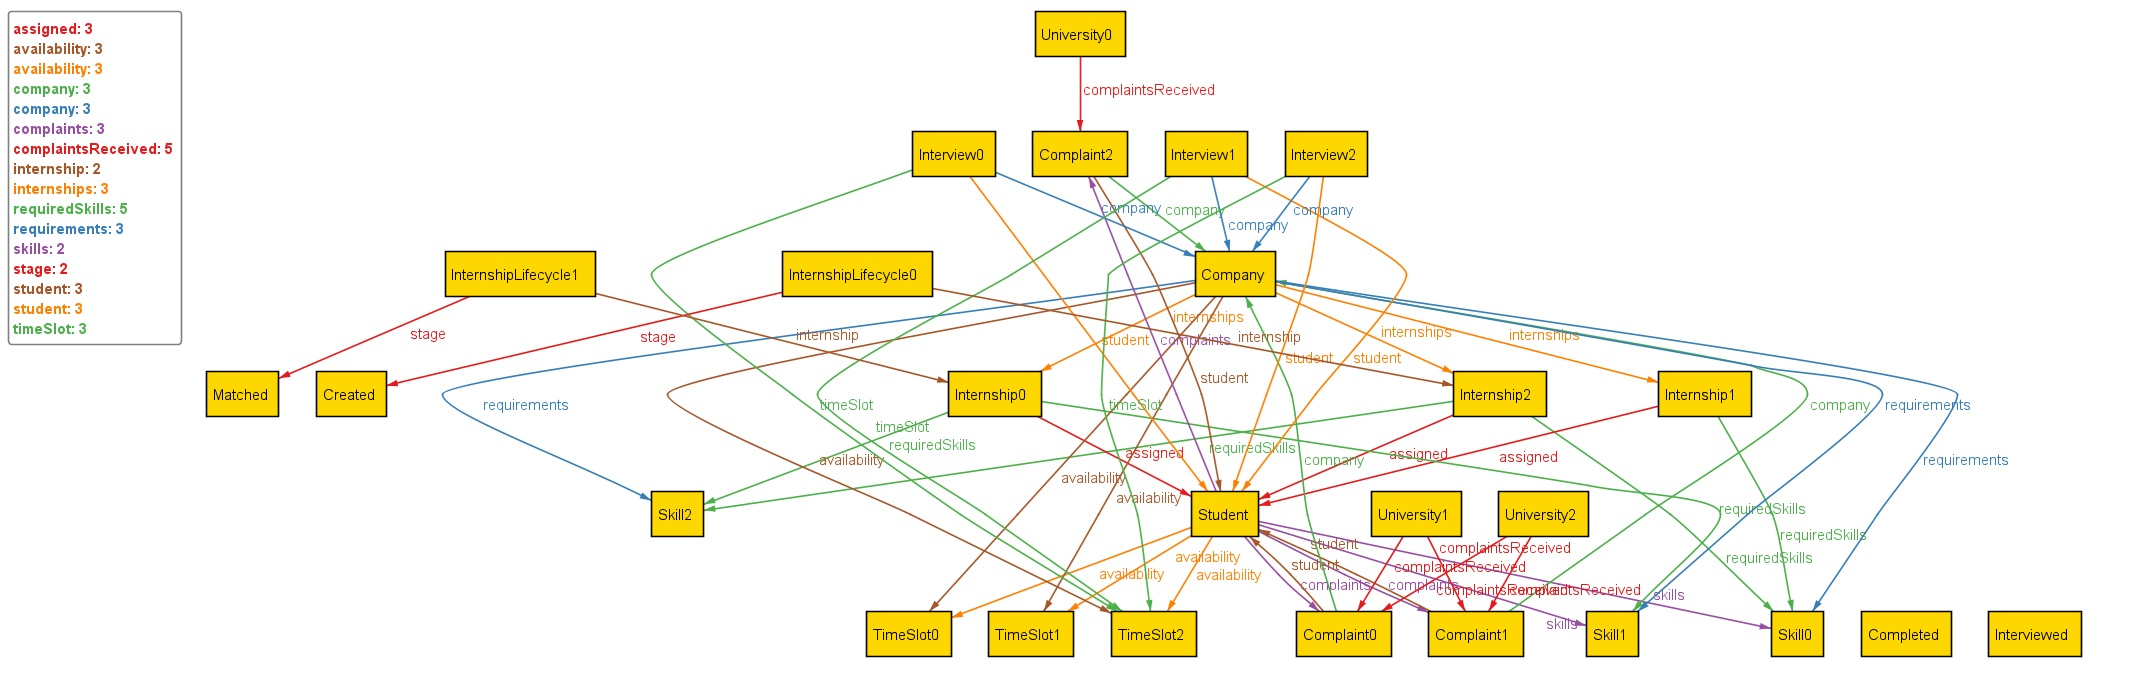
\includegraphics[height=0.25\textheight]{Images/Alloy2.jpg}}
\caption{\label{fig:metamodel}Alloy solver visualization for the UniqueAssignment predicate.}
\end{figure}


\begin{sidewaysfigure}
\centering
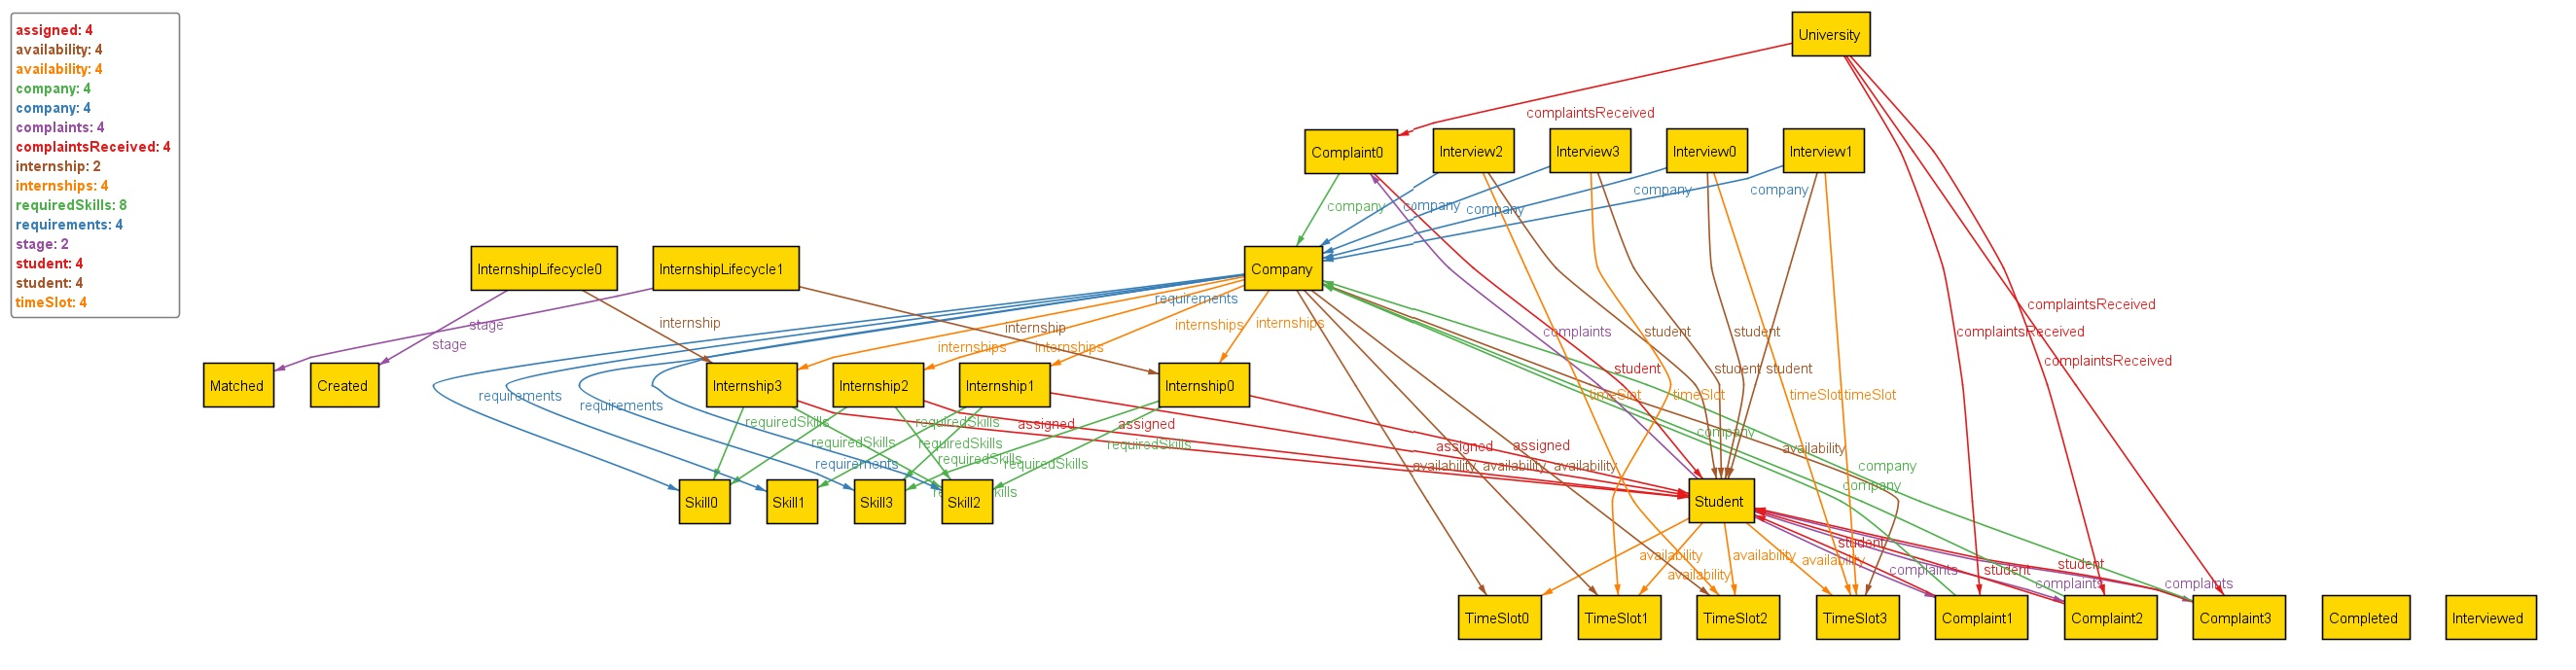
\includegraphics[width=\textwidth, angle=0]{Images/Alloy3.jpg}
\caption{\label{fig:metamodel}Alloy solver visualization for the ScheduleConflict predicate.}
\end{sidewaysfigure}

\begin{sidewaysfigure}
\centering
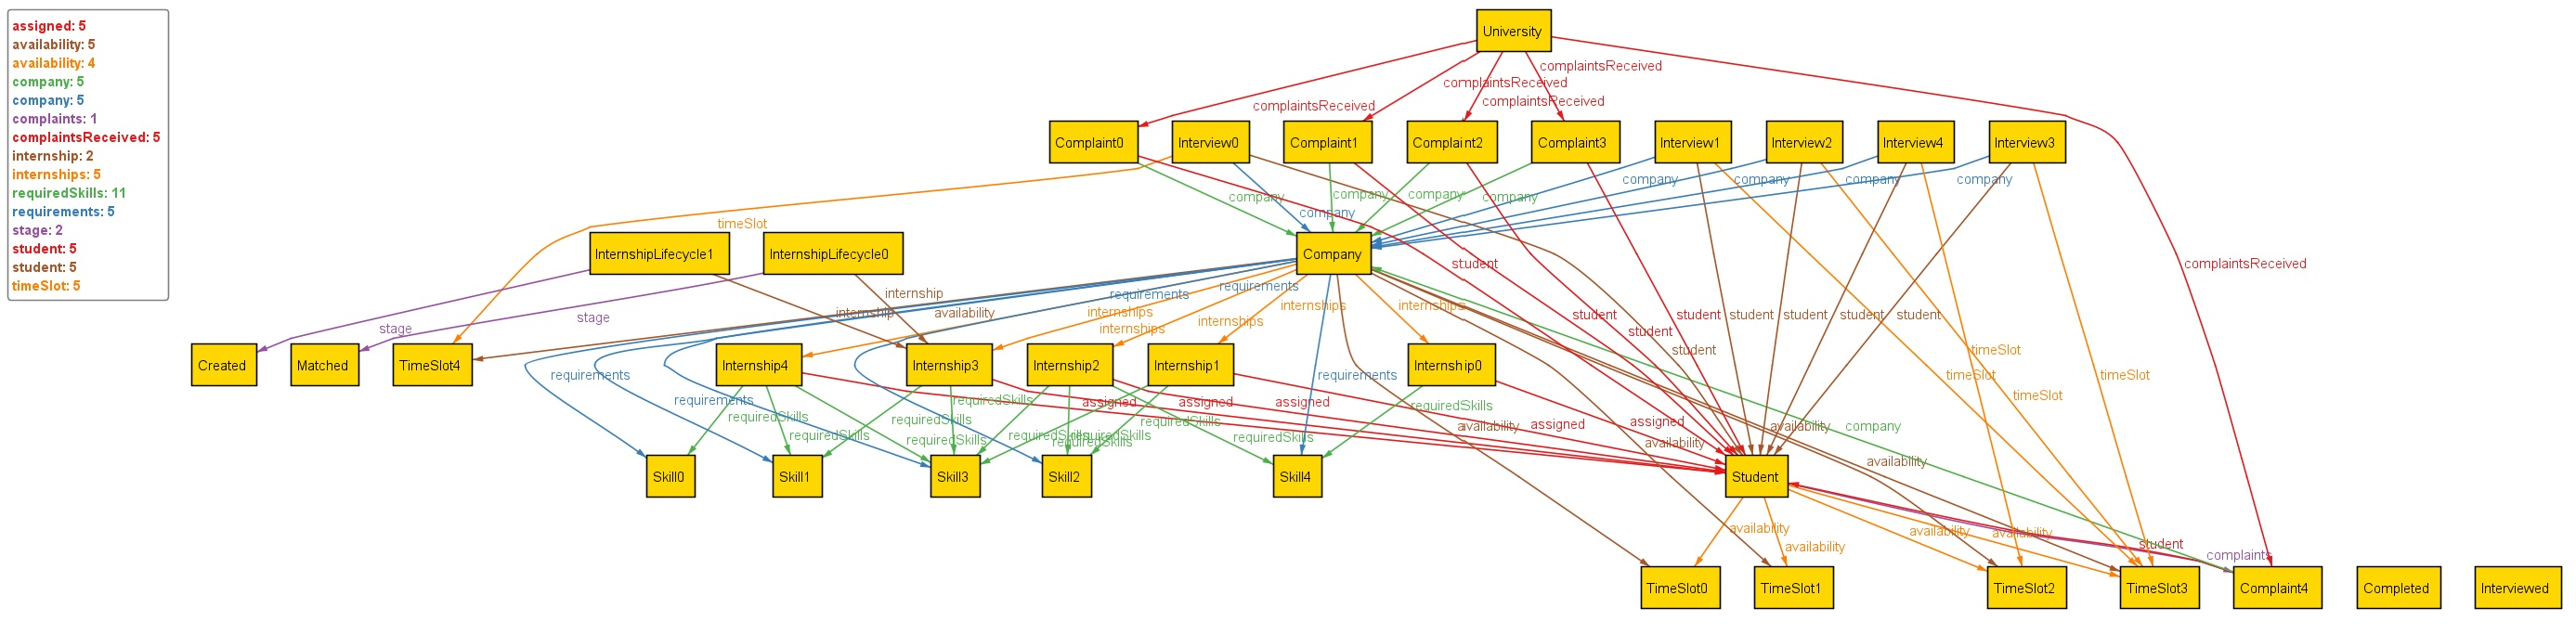
\includegraphics[width=\textwidth, angle=0]{Images/Alloy4.jpg}
\caption{\label{fig:metamodel}Alloy solver visualization for the ComplaintHandling predicate.}
\end{sidewaysfigure}

